% Created 2017-12-22 fre 18:31
% Intended LaTeX compiler: pdflatex
\documentclass{article}

%%%% settings when exporting code %%%% 

\usepackage{listings}
\lstset{
backgroundcolor=\color{white},
basewidth={0.5em,0.4em},
basicstyle=\ttfamily\small,
breakatwhitespace=false,
breaklines=true,
columns=fullflexible,
commentstyle=\color[rgb]{0.5,0,0.5},
frame=single,
keepspaces=true,
keywordstyle=\color{black},
literate={~}{$\sim$}{1},
numbers=left,
numbersep=10pt,
numberstyle=\ttfamily\tiny\color{gray},
showspaces=false,
showstringspaces=false,
stepnumber=1,
stringstyle=\color[rgb]{0,.5,0},
tabsize=4,
xleftmargin=.23in,
emph={anova,apply,class,coef,colnames,colNames,colSums,dim,dcast,for,ggplot,head,if,ifelse,is.na,lapply,list.files,library,logLik,melt,plot,require,rowSums,sapply,setcolorder,setkey,str,summary,tapply},
emphstyle=\color{blue}
}

%%%% packages %%%%%

\usepackage[utf8]{inputenc}
\usepackage[T1]{fontenc}
\usepackage{lmodern}
\usepackage{textcomp}
\usepackage{color}
\usepackage{enumerate}
\usepackage{graphicx}
\usepackage{grffile}
\usepackage{wrapfig}
\usepackage{capt-of}
\usepackage{rotating}
\usepackage{caption}
\usepackage{rotating}
\usepackage{longtable}
\usepackage{multirow}
\usepackage{multicol}
\usepackage{pdflscape}
\usepackage{setspace}
\usepackage{geometry}
\usepackage[normalem]{ulem}
\usepackage{amssymb}
\usepackage{amsmath}
\usepackage{amsfonts}
\usepackage{dsfont}
\usepackage{textcomp}
\usepackage{array}
\usepackage{ifthen}
\usepackage{hyperref}
\usepackage{natbib}
%
%%%% additional latex commands %%%%
%
%
%%%% additional packages %%%%
%
\usepackage{authblk}
\RequirePackage{amsmath}
\RequirePackage{algorithm}
\RequirePackage[noend]{algpseudocode}
\RequirePackage{fancyvrb}
\DefineVerbatimEnvironment{verbatim}{Verbatim}{fontsize=\small,formatcom = {\color[rgb]{0.5,0,0}}}
\RequirePackage{colortbl} % arrayrulecolor to mix colors
%% \input{0_Display.tex}
\RequirePackage{epstopdf} % to be able to convert .eps to .pdf image files
\RequirePackage{ifthen}
\RequirePackage{xspace} % space for newcommand macro
\RequirePackage{xifthen}
\RequirePackage{xargs}
\RequirePackage{dsfont}
\RequirePackage{amsmath,stmaryrd,graphicx}
\RequirePackage{prodint} % product integral symbol (\PRODI)
\newcommand\defOperator[7]{%
\ifthenelse{\isempty{#2}}{
\ifthenelse{\isempty{#1}}{#7{#3}#4}{#7{#3}#4 \left#5 #1 \right#6}
}{
\ifthenelse{\isempty{#1}}{#7{#3}#4_{#2}}{#7{#3}#4_{#1}\left#5 #2 \right#6}
}
}
\newcommand\defUOperator[5]{%
\ifthenelse{\isempty{#1}}{
#5\left#3 #2 \right#4
}{
\ifthenelse{\isempty{#2}}{\underset{#1}{\operatornamewithlimits{#5}}}{
\underset{#1}{\operatornamewithlimits{#5}}\left#3 #2 \right#4}
}
}
\newcommand{\defBoldVar}[2]{
\ifthenelse{\equal{#2}{T}}{\boldsymbol{#1}}{\mathbf{#1}}
}
\newcommandx\Cov[2][1=,2=]{\defOperator{#1}{#2}{C}{ov}{[}{]}{\mathbb}}
\newcommandx\Esp[2][1=,2=]{\defOperator{#1}{#2}{E}{}{[}{]}{\mathbb}}
\newcommandx\Prob[2][1=,2=]{\defOperator{#1}{#2}{P}{}{[}{]}{\mathbb}}
\newcommandx\Qrob[2][1=,2=]{\defOperator{#1}{#2}{Q}{}{[}{]}{\mathbb}}
\newcommandx\Var[2][1=,2=]{\defOperator{#1}{#2}{V}{ar}{[}{]}{\mathbb}}
\newcommandx\Binom[2][1=,2=]{\defOperator{#1}{#2}{B}{}{(}{)}{\mathcal}}
\newcommandx\Gaus[2][1=,2=]{\defOperator{#1}{#2}{N}{}{(}{)}{\mathcal}}
\newcommandx\Wishart[2][1=,2=]{\defOperator{#1}{#2}{W}{ishart}{(}{)}{\mathcal}}
\newcommandx\Likelihood[2][1=,2=]{\defOperator{#1}{#2}{L}{}{(}{)}{\mathcal}}
\newcommandx\Information[2][1=,2=]{\defOperator{#1}{#2}{I}{}{(}{)}{\mathcal}}
\newcommandx\Score[2][1=,2=]{\defOperator{#1}{#2}{S}{}{(}{)}{\mathcal}}
\newcommandx\Vois[2][1=,2=]{\defOperator{#1}{#2}{V}{}{(}{)}{\mathcal}}
\newcommandx\IF[2][1=,2=]{\defOperator{#1}{#2}{IF}{}{(}{)}{\mathcal}}
\newcommandx\Ind[1][1=]{\defOperator{}{#1}{1}{}{(}{)}{\mathds}}
\newcommandx\Max[2][1=,2=]{\defUOperator{#1}{#2}{(}{)}{min}}
\newcommandx\Min[2][1=,2=]{\defUOperator{#1}{#2}{(}{)}{max}}
\newcommandx\argMax[2][1=,2=]{\defUOperator{#1}{#2}{(}{)}{argmax}}
\newcommandx\argMin[2][1=,2=]{\defUOperator{#1}{#2}{(}{)}{argmin}}
\newcommandx\cvD[2][1=D,2=n \rightarrow \infty]{\xrightarrow[#2]{#1}}
\newcommandx\Hypothesis[2][1=,2=]{
\ifthenelse{\isempty{#1}}{
\mathcal{H}
}{
\ifthenelse{\isempty{#2}}{
\mathcal{H}_{#1}
}{
\mathcal{H}^{(#2)}_{#1}
}
}
}
\newcommandx\dpartiel[4][1=,2=,3=,4=\partial]{
\ifthenelse{\isempty{#3}}{
\frac{#4 #1}{#4 #2}
}{
\left.\frac{#4 #1}{#4 #2}\right|_{#3}
}
}
\newcommandx\dTpartiel[3][1=,2=,3=]{\dpartiel[#1][#2][#3][d]}
\newcommandx\ddpartiel[3][1=,2=,3=]{
\ifthenelse{\isempty{#3}}{
\frac{\partial^{2} #1}{\left( \partial #2\right)^2}
}{
\frac{\partial^2 #1}{\partial #2\partial #3}
}
}
\newcommand\Real{\mathbb{R}}
\newcommand\Rational{\mathbb{Q}}
\newcommand\Natural{\mathbb{N}}
\newcommand\trans[1]{{#1}^\intercal}%\newcommand\trans[1]{{\vphantom{#1}}^\top{#1}}
\newcommand{\independent}{\mathrel{\text{\scalebox{1.5}{$\perp\mkern-10mu\perp$}}}}
\author{Brice Ozenne, Julien Peron, \ldots{}, Marc Buyse}
\date{\today}
\title{BuyseTest: Assessing a treatment effect based on multiple outcomes using generalized pairwise comparisons}
\hypersetup{
 colorlinks=true,
 citecolor=[rgb]{0,0.5,0},
 urlcolor=[rgb]{0,0,0.5},
 linkcolor=[rgb]{0,0,0.5},
 pdfauthor={Brice Ozenne, Julien Peron, \ldots{}, Marc Buyse},
 pdftitle={BuyseTest: Assessing a treatment effect based on multiple outcomes using generalized pairwise comparisons},
 pdfkeywords={},
 pdfsubject={},
 pdfcreator={Emacs 26.0.50 (Org mode 9.0.4)},
 pdflang={English}
 }
\begin{document}

\maketitle
\lstset{language=r,label= ,caption= ,captionpos=b,numbers=none}
\begin{lstlisting}
library(BuyseTest)
\end{lstlisting}

\section{Functionalities}
\label{sec:org8e91f09}

\begin{center}
\begin{tabular}{ll}
Function & effect\\
\hline
simulBT & simulate outcomes for two groups of observations.\\
powerBT & power analysis using GPC.\\
constStrata & create a single strata variable from several categorical variables.\\
BuyseTest & perform GPC computations.\\
summary & display the output from GPC.\\
sensitivityBT & sensitivity analysis on choice of the thresholds of the GPC.\\
\end{tabular}
\end{center}



\section{Thresholds of clinical relevance}
\label{sec:org32d575b}

\subsection{Binary outcomes}
\label{sec:orga5a4361}

Thresholds are not relevant for binary variables. This is why it is
not possible to specify them through the formula interface. 

\bigskip

Internally, since binary outcomes are treated as continuous outcomes,
any threshold strictly small than 1 and strictly greater than 0 would
be valid. However to avoid confusion with the continuous case, only
thresholds equaling 1/2 are accepted. Specifying \texttt{NA} is also possible;
in such case the threshold will be automatically converted to \(1/2\).

\lstset{language=r,label= ,caption= ,captionpos=b,numbers=none}
\begin{lstlisting}
BuyseTest:::initThreshold(threshold = NA, type = 1, D = 1, endpoint = c("Y1"))
\end{lstlisting}

\begin{verbatim}
[1] 0.5
\end{verbatim}

This is because if \(Y=1\) and \(X=0\) then \(|Y-X| \geq 1/2\) 
while if \(Y=X\) then \(|Y-X| \leq 1/2\).

\subsection{Continuous and time to event outcomes}
\label{sec:orgb092f02}

Threshold for continuous outcomes must be strictly positive. Whenever
a threshold is set to 0, it will be automatically reassigned to \(10^{-12}\):
\lstset{language=r,label= ,caption= ,captionpos=b,numbers=none}
\begin{lstlisting}
BuyseTest:::initThreshold(threshold = 0, type = 2, D = 1, endpoint = c("Y1"))
\end{lstlisting}

\begin{verbatim}
[1] 1e-12
\end{verbatim}

This ensure that when \(Y=1\) and \(X=1.01\) then
\(|Y-X| \geq \tau=10^{-12}\) while whenever \(Y=X\) then \(|Y-X| \leq \tau=10^{-12}\)

\subsection{Time to event variables}
\label{sec:org0b0ea0a}


\begin{itemize}
\item cannot have twice the same pair (threshold, outcome)
\item thresholds corresponding to time to event variables must be decreasing
\end{itemize}


\begin{verbatim}
[1] 5e-01 1e-12 1e-12
\end{verbatim}

\section{Diagram}
\label{sec:org3e402f6}

\begin{center}
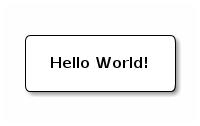
\includegraphics[width=.9\linewidth]{hello-world-round.png}
\end{center}
\end{document}